\chapter{Positivity Bounds}
\label{chap:positivity}

We will first study the elastic $2 \to 2$ scattering of identical massive scalar particles, described by the amplitude $\mathcal{M}(s,t,u)$. Our goal is to understand how general principles of quantum field theory constrain the low-energy behaviour of this amplitude, independently of the details of its ultraviolet (UV) completion.

At energies well below a cutoff scale $\Lambda$, the scattering process admits an effective field theory (EFT) description, in which the amplitude can be organized as a systematic expansion in powers of energy over $\Lambda$. The coefficients of this expansion encode the low-energy dynamics of the theory and are, in principle, arbitrary from the EFT point of view.

However, if the EFT arises from a consistent UV completion, its low-energy parameters cannot be completely unconstrained. In the following, we will assume that the underlying UV theory is causal, unitary and Lorentz invariant, while otherwise remaining agnostic about its microscopic structure. As we will see, these general assumptions imply non-trivial constraints on the analytic structure of the scattering amplitude, which in turn lead to positivity bounds on the EFT coefficients.


\section{Properties of the Scattering Amplitude}

As discussed in \autocite{Martin:1969ina}, the properties of the scattering of identical particles imply that the amplitude must be invariant under the exchange of the incoming and outgoing particles. In terms of Mandelstam variables, this invariance is implemented as a crossing symmetry under the interchange $ s \leftrightarrow u $.

Since the Mandelstam variables are not independent but satisfy
\begin{equation}
    s + t + u = 4m^2,
\end{equation}
it is convenient to work with only two independent variables. From now on, we define
\begin{equation}
    \mathcal{M}(s,t) \equiv \mathcal{M}\bigl(s,t,4m^2 - s - t\bigr).
\end{equation}

In addition, the scattering amplitude is assumed to be a real analytic function of the Mandelstam variables. Real analyticity implies that the values of the amplitude above and below the real axis are related through the Schwarz reflection principle. 
With this convention, real analyticity implies that, in the vicinity of the real axis,
\begin{equation}
    \mathcal{M}(s + i\varepsilon, t)
    = \mathcal{M}^*(s - i\varepsilon, t),
\end{equation}
while crossing symmetry further relates the amplitude at \(s\) to that at the crossed channel,
\begin{equation}
    \mathcal{M}(s + i\varepsilon, t)
    = \mathcal{M}^*\bigl(4m^2 - s - t + i\varepsilon, t\bigr).
    \label{eq:realan}
\end{equation}

Unitarity implies that the imaginary part of the scattering amplitude is strictly positive,
\begin{equation}
\Im\mathcal{M}(s) > 0.
\end{equation}
Moreover, unitarity leads to Froissart’s bound \autocite{PhysRev.123.1053}, which constrains the high-energy behavior of the amplitude. In particular, for fixed momentum transfer $t<0$ and sufficiently large center-of-mass energy $s$, the amplitude grows at most quadratically in $s$, so that
\begin{equation}
\lim_{s\to\infty} \frac{\mathcal{M}(s,t,u)}{s^{2}} = 0,
\end{equation}
when the limit is taken along lines of constant phase in the complex $s$-plane.


For fixed momentum transfer $t$, the scattering amplitude can be regarded as a complex function of the Mandelstam variable $s$. The general requirements of Lorentz invariance, causality and unitarity imply that $\mathcal{M}(s,t)$ is an analytic function of $s$ in the complex plane, except for singularities with a direct physical interpretation.

In the full theory, these singularities consist of isolated poles and branch cuts. Poles correspond to the exchange of single-particle states, while branch cuts arise from multi-particle production thresholds. For the scattering of identical scalar particles of mass $m$, the first branch cut in the $s$-channel starts at the two-particle threshold,
\begin{equation}
    s = 4m^2,
\end{equation}
and extends along the positive real axis to $s \to +\infty$. As a consequence of crossing symmetry, this cut is accompanied by a corresponding branch cut in the $u$-channel. When viewed as a function of complex $s$, and for fixed $t<0$, the amplitude therefore exhibits two branch cuts along the real axis: one for $s \geq 4m^2$, and another for $s \leq 4m^2 - t$.
At tree level, however, the amplitude does not exhibit branch cuts, as no multi-particle intermediate states can go on shell. 

In an effective field theory, the amplitude is only expected to provide a valid description below a cutoff scale $\Lambda^2$, with $\Lambda^2 \geq 4m^2$. For the purposes of dispersion relations, however, one assumes that the full analytic structure of the amplitude is inherited from a consistent UV completion. In particular, the branch cuts associated with particle production are taken to lie above the EFT regime, so that the low-energy expansion is valid away from the cuts, while their presence controls the analytic structure needed to write dispersion relations. We will therefore assume that the first branch point lies at or above the cutoff scale $\Lambda^2$.

\subsection{Low-Energy Expansion}

Since the scattering amplitude is analytic at low energies, it admits a low-energy expansion that can be computed within an effective field theory valid below a cutoff scale. At tree level, and assuming that the EFT is weakly coupled up to the cutoff of the theory $\Lambda^2$, the amplitude can be written as the most general function symmetric under permutations of $s$, $t$ and $u$. In the case in which there is no exchange of other particles, the amplitude is
\begin{eqnarray}
    \mathcal{M}_{\text{low}}(s,t,u) = - \lambda 
     + g_2 (s^2 + t^2 + u^2) + g_3 (stu) + g_4 (s^2 + t^2 + u^2)^2 \notag \\ + g_5 (s^2 + t^2 + u^2)(stu) 
    + g_6 (s^2 + t^2 + u^2)^3 +\notag \\ g_6'(stu)^2 + g_7 (s^2 + t^2 + u^2)^2(stu) + \cdots \,
    \label{eq:eft} 
\end{eqnarray}

\subsection{High-Energy Expansion}

At high energies, we will expand the scattering amplitude in partial waves as
\begin{equation}
    \mathcal{M}(s,t,u)
    =
    \sum_{\substack{J \,\text{even}}}
    16\pi(2J+1)\,
    \mathcal{P}_J\left(1+\frac{2t}{s-4m^2}\right)
    f_J(s),
\end{equation}
where $\mathcal{P}_J(x)$ denote the Legendre polynomials, and all the dynamical information of the process is encoded in the partial-wave amplitudes $f_J(s)$.

The amplitude $\mathcal{M}$ is related to the $S$-matrix through
\begin{equation}
    S = 1 + i\,\mathcal{M}.
\end{equation}
Projecting onto definite angular momentum, we define
\begin{equation}
    S_J(s) = 1 + i\, f_J(s).
\end{equation}
Unitarity of the $S$-matrix then implies the constraint
\begin{equation}
    |S_J(s)| \leq 1.
\end{equation}

Introducing the spectral density
\begin{equation}
    \rho_J(s) \equiv \Im f_J(s),
\end{equation}
the imaginary part of the full amplitude, which will play a central role in what follows, can be written as
\begin{equation}
    \Im \mathcal{M}(s,t,u)
    =
    \sum_{\substack{J \,\text{even}}}
    16\pi(2J+1)\,
    \mathcal{P}_J\left(1+\frac{2t}{s-4m^2}\right)
    \rho_J(s).
    \label{eq:highendecomp}
\end{equation}

\begin{Todo}
Comprobar raíz
\end{Todo}
    

Finally, the unitarity condition on the $S$-matrix translates into the following bounds on the spectral densities:
\begin{equation}
    0 \leq \rho_J(s) \leq 2,
    \qquad \forall\, s > 0,\ \forall\, J \ \text{even}.
\end{equation}
In particular, from now on we will make extensive use of the fact that the functions $\rho_J(s)$ are positive definite. We remark that this is a consequence of the unitarity of the $S$ matrix, and will remain true even if we do not know any more information about the amplitude at high energies.

\section{Dispersion Relations}
\label{sec:dispersion}
We start by defining the $n-$substracted arc as \autocite{Caron-Huot:2020cmc}
\begin{equation}
    a_n(t) = \frac{1}{2 \pi i} \oint_\mathcal{C} \frac{ds}{s-2m^2} \frac{\mathcal{M}(s, t)}{[(s-2m^2)(s+t-2m^2)]^{n/2}},
\end{equation}
where $\mathcal{C}$ is the contour shown in figure 
\begin{Todo}
    Añadir figura
\end{Todo}
. For simplicity, from now on we will define the crossing symmetric variable $\hat{s} = s-2m^2$.
The integrand is analytic inside the contour except for the poles on the real axis, that come both from the poles that are present in the amplitude and the ones that arise from the denominator. Thus, from Cauchy's residue theorem, we can write that 
\begin{equation}
    a_n(t) = \sum_{\hat{s}_i \in \mathbb{R}} 
    \Res_{\hat{s} = \hat{s}_i} \left[
    \frac{\mathcal{M}(\hat{s},t)}{\hat{s} [\hat{s}(\hat{s}+t)]^{n/2}}
    \right],
    \label{eq:residues}
\end{equation}
where $\hat{s}_i$ denote the values of $\hat{s}$ for which the integrand has poles inside the contour $\mathcal{C}$. Because all these poles are at energies below the cutoff of the theory, it is posible to calculate expressions for the arcs within the EFT, this is, by using the $\mathcal{M}_\text{low}$ given by~\Cref*{eq:eft}.

It is also possible to compute the coefficients \( a_n(t) \) by evaluating the contour integral explicitly. The result can be written as
\begin{equation}
    a_n(t)
    =
    \frac{1}{2\pi i}
    \left(
        \int_{\cap_\infty}
        + \int_{l_1}
        + \int_{\tilde{l}_1}
        + \int_{l_2}
        + \int_{\tilde{l}_2}
        +  \int_{\cap_{-\infty}}
    \right) \frac{d\hat{s}}{\hat{s}}
    \frac{\mathcal{M}(\hat{s},t)}{[\hat{s}(\hat{s}+t)]^{n/2}} \, .
\end{equation}
For sufficiently large values of \( |s| \), Froissart’s bound ensures that, for $n \geq 2$, the scattering amplitude grows at most polynomially. As a consequence, the contributions from the portions of the contour taken to infinity vanish. In particular, one finds
\begin{equation}
    \int_{\cap_\infty} \frac{d\hat{s}}{\hat{s}}
    \frac{\mathcal{M}(\hat{s},t)}{[\hat{s}(\hat{s}+t)]^{n/2}}
    =
    \int_{\cap_{-\infty}} \frac{d\hat{s}}{\hat{s}}
    \frac{\mathcal{M}(\hat{s},t)}{[\hat{s}(\hat{s}+t)]^{n/2}}
    =
    0 .
\end{equation}
Thus, taking into account \Cref*{eq:realan} together with crossing symmetry, we have that 
\begin{equation}
   a_n(t) = \frac{2}{\pi }\int_{\Lambda^2-2m^2}^{\infty} \frac{d \hat{s}}{\pi \hat{s}} \frac{2\hat{s}+t}{\hat{s}+t} \frac{\Im \mathcal{M}(\hat{s},t) }{[\hat{s}(\hat{s}+t)]^{n/2}} 
   \label{eq:highen}
\end{equation}

This result is remarkable, as it provides a second, independent way of computing the coefficients \( a_n(t) \). On the one hand, the expression in \Cref*{eq:residues} depends exclusively on low-energy information encoded in the effective field theory. On the other hand, \Cref*{eq:highen} involves only the imaginary part of the amplitude at energies above the EFT cutoff \( \Lambda \), and therefore probes the unknown ultraviolet completion of the theory.

\begin{Todo}
    Añadir algo de superluminalidad?
\end{Todo}

\subsection{Sum rules}
\label{sec:sumrules}

Inserting in the expansion from \Cref*{eq:highendecomp}, the arcs can be rewritten as 
\begin{eqnarray}
    a_n(t) = \sum_{J \text{ even}} \int_{\Lambda^2-2m^2}^{\infty} \frac{d\hat{s}}{\hat{s}}  32  (2 J + 1) \mathcal{P}_J \left( 1 + \frac{2t}{\hat{s}-2m^2} \right) \frac{2\hat{s}+t}{\hat{s}+t}\frac{\rho_J(\hat{s})}{[\hat{s}(\hat{s}+t)]^{n/2}}.
\end{eqnarray}
It is convenient to introduce the following high-energy average of a function $F(s,J)$:
\begin{eqnarray}
    \langle F(\hat{s},J) \rangle
    \equiv
    \sum_{J \text{ even}} 32   (2J+1)\, \int_{\Lambda^2-2m^2}^{\infty} \frac{d\hat{s}}{\hat{s}} \; 
    \rho_J(\hat{s})\, F(\hat{s},J).
\end{eqnarray}

Unitarity implies that $\rho_J(s)\geq 0$ for all $\hat{s}\geq\Lambda^2-2m^2>0$ and even $J$. Therefore, the average
$\langle F(\hat{s},J)\rangle$ defines a positive linear functional. In particular, if
$F(\hat{s},J)\geq 0$ for all $\hat{s}\geq\Lambda^2-2m^2>0$ and even $J$, then
\begin{eqnarray}
    \langle F(\hat{s},J) \rangle \geq 0 .
\end{eqnarray}

With this notation, the arcs  can be compactly written as
\begin{equation}
    a_n(t)
    =
    \left\langle
    \frac{2\hat{s}+t}{\hat{s}+t}
    \frac{
        \mathcal{P}_J\left(1+\frac{2t}{\hat{s}-2m^2}\right)
    }{
        [\hat{s}(\hat{s}+t)]^{n/2}
    }
    \right\rangle
    \;\geq\; 0 \, .
\end{equation}

To better appreciate the power of this result, we now compute the arcs explicitly for the EFT introduced in \Cref{eq:eft}. For simplicity, we focus on the $2 \rightarrow 2$ scattering of massless scalars. Using \Cref*{eq:residues}, we obtain
\begin{equation}
a_2 = 2g_2 - g_3 + 8 g_4 t^2 + \cdots
= \left\langle \frac{(2s+t)\mathcal{P}_J\left(1+\frac{2t}{s}\right)}{s (s+t)^2} \right\rangle ,
\end{equation}
\begin{equation}
a_4 = 4g_4 + \cdots
= \left\langle \frac{(2s+t)\mathcal{P}_J\left(1+\frac{2t}{s}\right)}{s^2 (s+t)^3} \right\rangle .
\end{equation}
For $t \ll \Lambda^2$, the Legendre polynomials admit the expansion
\begin{equation}
\mathcal{P}_J\left(1+\frac{2t}{s}\right)
\simeq
1
+ J(J+1)\frac{t}{s}
+ \frac{1}{4}(J-1)J(J+1)(J+2)\frac{t^2}{s^2}
+ \cdots .
\end{equation}
Matching the left- and right-hand sides of the arcs order by order in $t$, the Wilson coefficients can be expressed as heavy averages,
\begin{equation*}
g_2 = \left\langle \frac{1}{s^2} \right\rangle,
\qquad
g_3 = \left\langle \frac{3 - 2J(J+1)}{s^3} \right\rangle,
\end{equation*}
\begin{equation*}
g_4 = \left\langle \frac{1}{2s^4} \right\rangle
= \left\langle
\frac{1 - J(J+1) + \tfrac{1}{8} J^2 (J+1)^2}{2 s^4}
\right\rangle .
\end{equation*}

There are some important observations than can now be made from these expresions.
First, since $s^2 > 0$ and $s^4 > 0$ inside the heavy averages, it immediately follows that
\begin{equation}
g_2 > 0,
\qquad
g_4 > 0.
\end{equation}
No analogous positivity statement can be made for $g_3$, because its numerator depends on the spin $J$ and is not positive definite.
Nevertheless, we can bound it from above:
\begin{equation}
g_3
= \left\langle \frac{3 - 2J(J+1)}{s^3} \right\rangle
\leq
\left\langle \frac{3}{s^3} \right\rangle ,
\end{equation}
since $3 - 2J(J+1) \leq 3$ for all $J$.
Because in the heavy averages we have $s \geq \Lambda^2$, it follows that
\begin{equation}
\frac{1}{s^3} \leq \frac{1}{\Lambda^2}\frac{1}{s^2}.
\end{equation}
Therefore,
\begin{equation}
g_3
\leq
\left\langle \frac{3}{s^3} \right\rangle
\leq
\frac{1}{\Lambda^2}
\left\langle \frac{3}{s^2} \right\rangle
= \frac{3 g_2}{\Lambda^2}.
\end{equation}
Similarly,
\begin{equation}
g_4
= \left\langle \frac{1}{2 s^4} \right\rangle
\leq
\frac{1}{\Lambda^4}
\left\langle \frac{1}{2 s^2} \right\rangle
= \frac{g_2}{2 \Lambda^4}.
\end{equation}

Second, we observe that we have obtained two different heavy-average representations for the same Wilson coefficient $g_4$. Although the integrands differ, their averages must coincide. It therefore follows that
\begin{equation}
0 = \left\langle
\frac{J(J+1)-\tfrac{1}{8}J^2 (J+1)^2}{s^4}
\right\rangle .
\end{equation}

\subsection{Null Constraints}

What we have just encountered is the first example of what are known as 
\textbf{null constraints}. These are relations of the form
\begin{equation}
    \left\langle \mathcal{F}(s,J) \right\rangle = 0,
\end{equation}
where the integrand $\mathcal{F}(s,J)$ is not identically zero, but its heavy 
average vanishes once integrated against the positive spectral measure.


Since the heavy-average measure is positive, a vanishing average of a 
non-trivial function imposes non-trivial restrictions on the spectral densities 
$\rho_J(s)$ entering the measure. In particular, the spin-dependent 
contributions must combine in such a way that their weighted integral vanishes. 
Null constraints therefore restrict the allowed distribution of heavy states in 
spin and mass.

Moreover, null constraints play a crucial role in deriving bounds on Wilson 
coefficients. Because the Wilson coefficients themselves are given by positive 
heavy averages of specific kernels, the existence of vanishing averages for 
related kernels allows one to relate or eliminate certain spin contributions. 
As a result, one can derive non-trivial upper and lower bounds on the EFT 
couplings.

\subsection{Systematic Null Constraints from Crossing Symmetry}
For a single identical massless scalar, crossing symmetry implies
\begin{equation}
\mathcal{M}(s,t) = \mathcal{M}(t,s).
\end{equation}
This symmetry can be encoded in a contour integral representation for the null constraints:
\begin{equation}
\oint_0 \frac{dt}{2 \pi i} \oint_\infty \frac{ds}{2 \pi i}
\frac{\mathcal{M}(s, t)}{st} \left(
\frac{1}{s^m t^n} - \frac{1}{s^n t^m}
\right) = 0,
\label{eq:hihgenint}
\end{equation}
where $m, n \geq2$, the $t$-contour encircles the origin, and the $s$-contour encircles infinity.
The intuition is that this integral projects out the coefficients in the low-energy expansion corresponding to the combination $s^m t^n - t^m s^n$.
Expanding the low-energy amplitude in a Taylor series around $s=t=0$,
\begin{equation}
\mathcal{M}_\text{low}(s,t) = \sum_{k,l \ge 0} a_{kl} s^k t^l,
\end{equation}
crossing symmetry enforces
\begin{equation}
a_{mn} - a_{nm} = 0.
\end{equation}
Thus, the low-energy contributions to \Cref{eq:hihgenint} vanish identically, leaving only contributions from the high-energy part, $\mathcal{M}_{\text{high}}$.
Using the same contour deformation arguments as in the derivation of the sum rules, the integral can then be rewritten as an integral along the branch cuts.
Evaluating the integral using the residue theorem and projecting onto spin $J$ partial waves, we find the null constraints
\begin{equation}
\left\langle \Res_{t=0} \left[ \mathcal{P}_J \left( 1+ \frac{2t}{s} \right)
\left( \frac{1}{s^m t^n } - \frac{1}{ s^n t^m} - \frac{(-1)^m}{(s+t)^m t^n} + \frac{(-1)^n}{(s+t)^n t^m} \right) \right] \right\rangle = 0.
\end{equation}

These null constraints form a systematic set of relations that can be explicitly computed for fixed $m$ and $n$, for instance using symbolic software such as Mathematica. While the procedure generates a large number of constraints, it is important to note that some of them may be linearly dependent of others.

\section{Finding Bounds on the Coefficients}
So far, we have seen that the unitarity and analyticity of the scattering amplitude allow us to express the Wilson coefficients of our low-energy effective field theory as weighted averages over heavy states, in which only contributions from the UV completion appear. In general, we will write 
\begin{equation}
    g_n = \langle g_n(s, J) \rangle.
\end{equation}

Moreover, we have identified a set of null constraints, which satisfy
\begin{equation}
\langle n_i(s, J) \rangle = 0.
\end{equation}
As discussed earlier, these null constraints impose nontrivial conditions on the measure defining the weighted averages. Our next goal is to determine the range of values for the Wilson coefficients that are consistent with these constraints. To do this, we will rephrase our problem as a positive semidefinite optimization problem, which can be solved numerically.

As a concrete example, let us consider the problem of bounding the ratio
\[
\tilde{g}_n \equiv \frac{g_n}{g_2},
\]
where $g_n$ and $g_2$. Our goal is to find rigorous lower or upper bounds on $\tilde{g}_n$.

We introduce a vector of functions that includes the relevant quantities as well as a finite set of null constraints:
\[
\vec{v}(s,J) = \big(g_2(s,J),\ g_n(s,J),\ n_1(s,J), \dots, n_l(s,J) \big),
\]
where
$g_2(s,J)$ and $g_n(s,J)$ are the functions we want to relate and $n_i(s,J)$ are null constraints.

We also define a corresponding vector of coefficients:
\[
\vec{c} = \big(-A, 1, c_1, \dots, c_l \big),
\]
where $A$ and the $c_i$ are parameters to be determined.  


Using these vectors, we define the linear combination
\[
F(s,J) \equiv \vec{c} \cdot \vec{v}(s,J) 
= -A \, g_2(s,J) + g_n(s,J) + \sum_{i=1}^l c_i\, n_i(s,J).
\]
By construction, the heavy average of $F$ over $s$ and $J$ satisfies
\[
\langle F(s,J) \rangle = -A \, g_2 + g_n,
\]
since the null constraints vanish on average: $\langle n_i(s,J) \rangle = 0$.  
If we can choose coefficients $A$ and $c_i$ such that 
\[
F(s,J) \ge 0 \quad \text{for all } s,J,
\]
then its average also satisfies $\langle F(s,J) \rangle \ge 0$, which implies
\[
-A \, g_2 + g_n \ge 0 \quad \Rightarrow \quad \frac{g_n}{g_2} \ge A,
\]
assuming $g_2 \ge 0$.  

By maximizing $A$ under the positivity condition on $F(s,J)$, we obtain the optimal lower bound for the ratio $\tilde{g}_n$. 

Similarly, we can also find an upper bound for $\tilde{g}_n$. To do so, we define a new vector of coefficients 
\begin{equation}
    \vec{c}{\;'}(s,t) = (B, -1, c'_1, \ldots, c'_l).
\end{equation}
Now, 
\begin{equation}
    \langle F'(s, J) \rangle = Bg_2 - g_n \geq 0 \Rightarrow \tilde{g}_n \leq B.
\end{equation}
By minimizing $B$ keeping the positivity condition on $F'(s,J)$ we find the optimal upper bound for $\tilde{g}_n$.

Problems of this type can be formulated as semidefinite programs and solved numerically using the \texttt{SDPB} solver (\autocite{Simmons-Duffin:2015qma}, \autocite{Landry:2019qug}). In practice, \texttt{SDPB} takes as input a set of polynomial matrices whose positivity must be enforced over a given domain and returns the optimal value of a linear objective function subject to these positivity constraints.

To implement this procedure numerically, we must introduce a truncation. First, we retain only a finite number of null constraints. Second, the positivity condition must hold for all even spins $J$, but numerically we can only impose it up to a maximum value $J_{\text{max}}$. In addition, to improve convergence, it is useful to include constraints at parametrically large values of $J$, such as $100\,J_{\text{max}}$ or even $10^5\,J_{\text{max}}$. As we will discuss in later sections, the inclusion of sufficiently large spin values is crucial for achieving convergence.

\begin{Todo}
Explain more?
\end{Todo}
    

For $g_3$ we find that 
\begin{equation}
   -5.31 \leq  \frac{ \Lambda^2 g_3}{g_2} \leq 1.5.
\end{equation}

Moreover, this numerical approach can be extended to study the allowed regions in planes defined by pairs of Wilson coefficients. For instance, consider the $(\tilde{g}_3, \tilde{g}_4)$ plane. We start by fixing the allowed range of $\tilde{g}_3$ (which we just determined). Our function vector will now be 
\begin{equation}
    \vec{v}(s, J) = (g_2(s,J), \Lambda^2 g_3(s,J), \Lambda^4 g_4(s,J), \vec{n}_i),
\end{equation}
and the coefficient vector is 
\begin{equation}
    \vec{c} = (-A, -B, 1, \vec{c}_i).
\end{equation}
Therefore,
\begin{equation}
    \langle F(s,J) \rangle = -A g_2 - B \Lambda^2 g_3 + \Lambda^4 g_4 \geq 0 \Rightarrow \tilde{g}_4 \geq A + B \tilde{g}_3.
\end{equation}
Choosing a $\tilde{g}_3^0$ in the allowed range, 
\begin{equation}
    \tilde{g}_4 \geq A + B \tilde{g}_3^0. 
\end{equation}
Maximizing $A + B \tilde{g}_3^0$, we find the optimal lower bound for $\tilde{g}_4$. A similar procedure can be done to find the optimal upper bound. \Cref{fig:g3g4} show the results found numerically for the allowed region of these two coefficients.

\begin{figure}[hbtp]
    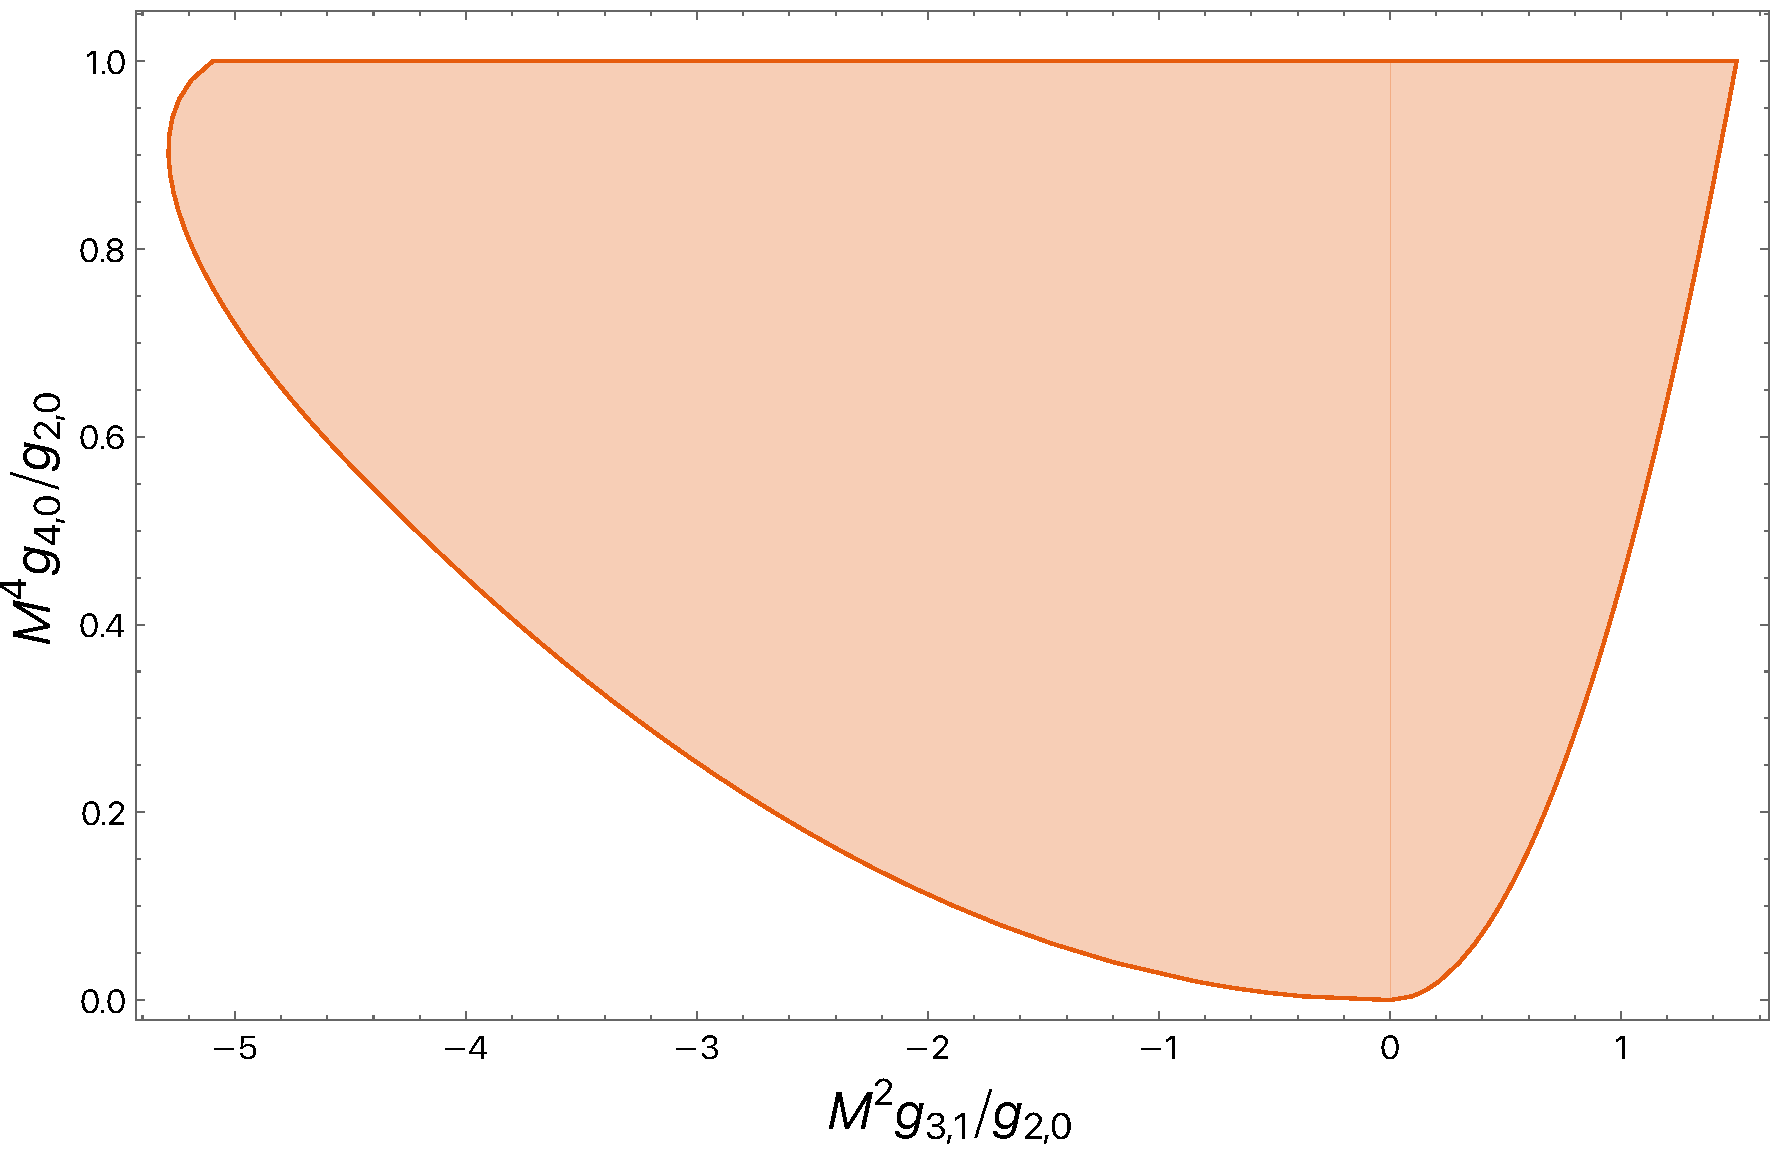
\includegraphics[width = 0.7 \textwidth]{ figures/g3g4.pdf}
    \caption{Allowed region for the $\tilde{g}_3$ and $\tilde{g}_4$ Wilson coefficient in a theory for a massless scalar.}
    \label{fig:g3g4}
\end{figure}

\section{Adding Resonances}
\label{sec:res}
Having established how to constrain the allowed parameter space of the Wilson coefficients in an EFT, we now turn to a different question. Suppose we extend the theory by allowing the exchange of intermediate resonances with mass $m_i$ and spin $J_i$.

The presence of such a state modifies the analytic structure of the amplitude by introducing additional poles. In particular, the propagator of the intermediate particle generates a pole at $s=m_i^2$, while crossing symmetry implies a corresponding pole at $s = -m_i^2 - t$.
In the vicinity of the poles, the amplitude factorizes and takes the universal form \autocite{Huang:2025icl}
\begin{equation}
    \mathcal{M}(s,t)|_{s \to m_i^2} \sim -\frac{\lambda_i^2 \mathcal{P}_{J_i}\left(1 + \frac{2t}{s}\right)}{s - m_i^2},
\end{equation}
with $\lambda_i^2 \geq 0$. Our goal is to derive an upper bound on $\lambda_i^2$. This is particularly interesting, as it will provide further insight into the structure the spectrum in these theories. If the upper bound on $\lambda_i^2$ vanishes, it would imply that our scalar cannot couple to the $i$-th resonance respecting unitarity and positivity.

A possible approach to achieve this would be to repeat the analysis performed in \Cref{sec:dispersion}. First, one would explicitly write down the amplitude including the exchange of the resonances. Next, one would compute the corresponding arcs for this modified amplitude, which will now depend both on the Wilson coefficients and on the resonance couplings $\lambda_i^2$, and relate them to the appropriate heavy averages. Finally, one would combine the arcs in such a way that the contributions proportional to the Wilson coefficients cancel, yielding dispersion relations for the couplings.

There is, however, a more elegant approach to this new problem. Instead of treating the resonance exchange explicitly within the low-energy amplitude and repeating the full dispersive analysis, we will regard the new poles introduced by the resonances as part of the high-energy contribution to the dispersion relations. In this framework, we use the fully analytic amplitude in \Cref{eq:eft}. The high-energy spectrum is then modeled as consisting of isolated poles together with a continuum that sets in above a scale $\Lambda'\.^2$, as shown in figure.
\begin{Todo}
Añadir figura
\end{Todo}
    

This separation allows us to keep the low-energy expansion unchanged, while encoding the resonance effects directly in the high-energy spectral density, which is modified as 
\begin{equation}
    \rho_J(s) \longrightarrow \rho'_J(s) + \sum_i \delta_{J, J_i} \lambda_i^2 \delta(s-m_i^2).
\end{equation}
Thus, the heavy average of a certain function is modified as 
\begin{equation}
    \langle F(s, J) \rangle \longrightarrow \langle F(s, J) \rangle' +\sum_{i}  \lambda_i^2 F(m_i^2, J),
\end{equation}
where $\langle \rangle' $ indicates a heavy average taken with the measure defined by $\rho'_J$.

For example, including only one resonance with mass $m_r$, spin $J_r$ and coupling $\lambda_r^2$,
\begin{equation}
    g_2 = \left\langle \frac{1}{s^2} \right\rangle' + \frac{\lambda_r^2}{m_r^4}.
\end{equation}
We will now see how to use this to bound $\lambda_r^2$. Similarly as before, we start by defining our vector of functions as 
\begin{equation}
    \vec{v}(s,J) = \left(0, \; g_2(s,J), \; \vec{n}(s, J) \right).
\end{equation}
We can define another vector, $\vec{v}_r$, as 
\begin{equation}
    \vec{v}_r  =  \left(-\frac{1}{m_r^4}, \; g_2(m_r^2,J_r),  \; \vec{n}(m_r^2, J_r) \right).
\end{equation}
If our vector of coefficients is 
\begin{equation}
    \vec{c} = (\;1, A, \vec{d}\;),
\end{equation}
we have that 
\begin{equation}
    \vec{c} \cdot \vec{v}_r = - \frac{1}{m_r^4} + \lambda_r^2  \;  \frac{A}{m_r^4} + \lambda_r^2 \; \vec{d} \cdot \vec{n}(m_r^2, J_2).
\end{equation}
and that
\begin{equation}
    \langle \vec{c} \cdot  \vec{v}(s, J) \rangle =  A g_2 =  \langle\vec{c} \cdot \vec{v}(s, J) \rangle'  + \lambda_r^2  \;  \frac{A}{m_r^4} + \lambda_r^2 \; \vec{d} \cdot \vec{n}(m_r^2, J_r).
\end{equation}
This can be rewritten as 
\begin{equation}
    Ag_2 - \frac{\lambda_r^2}{m_r^4} =  \langle\vec{c} \cdot \vec{v}(s, J) \rangle' \underbrace{ - \frac{\lambda_r^2}{m_r^4} + \lambda_r^2  \;  \frac{A}{m_r^4} + \lambda_r^2 \; \vec{d} \cdot \vec{n}_i(m_r^2, J_r)}_{\vec{c}\cdot \vec{v}_r}
\end{equation}
Imposing that $ \vec{c} \cdot \vec{v}(s, J)  \geq 0$ and that $\vec{c}\cdot \vec{v}_r \geq 0$, and using that $g_2 \geq 0$, this becomes 
\begin{equation}
    A \geq \frac{\lambda_r^2}{g_2 m_r^4}. 
    \label{eq:coupling}
\end{equation}
Thus, by minimizing $A$ keeping the positivity conditions, we find the optimal upper bound on $\lambda_r^2$.

This can be generalized for a system with more resonances, with mass $m_i$ and spin $J_i$. Suppose that we want to study the maximum value of the coupling $\lambda_k^2$.  The $\vec{v}(s,J)$ and $\vec{c}$ vectors are defined in the same way as before. Additionally, we have that 
\begin{equation}
    \vec{v}_i = \left(0, \; g_2(m_i^2,J_i),  \; \vec{n}(m_i^2, J_i) \right) \text{ for } j \neq k
\end{equation}
and 
\begin{equation}
    \vec{v}_k = \left(-\frac{1}{m_k^4}, \; g_2(m_k^2,J_k),  \; \vec{n}_i(m_k^2, J_k) \right).
\end{equation}
Imposing that $\vec{c} \cdot \vec{v}(s,J) \geq 0$, $\vec{c} \cdot \vec{v}_k \geq 0$ and $\vec{c} \cdot \vec{v}_j \geq 0$, we arrive again at the condition from \Cref*{eq:coupling} for $\lambda_k^2$. Minimizing $A$ we will find the optimal upper bound for this coupling.
\subsection{Generalization to Massive Scalars}

The previous analysis can be straightforwardly extended to the $2 \rightarrow 2$ scattering of a scalar field with mass $m$. In this case, the exchange of a resonance of mass $m_r$ introduces poles in the $s$-channel amplitude at
\[
s = m_r^2
\quad \text{and} \quad
s = 4m^2 - m_r^2,
\]
for fixed $t = 0$, as required by crossing symmetry.

Introducing the crossing-symmetric variable
\[
\hat{s} = s - 2m^2,
\]
these poles are located at
\[
\hat{s} = m_r^2 - 2m^2
\quad \text{and} \quad
\hat{s} = 2m^2 - m_r^2,
\]
which can be compactly written as
\[
\hat{s} = \pm \abs{m_r^2 - 2m^2}.
\]

Therefore, depending on the sign of $m_r^2 - 2m^2$, only one of these poles contributes to the high-energy average, as shown in figure 
\begin{Todo}
    Añadir figura 
\end{Todo}
. The procedure described in the previous section applies without modification, the only required change being the replacement
\[
\delta(s - m_r^2) \;\longrightarrow\; 
\delta\big(s - \abs{m_r^2 - 2m^2}\big).
\]


\section{Different Numbers of Subtractions}

So far, we have focused on amplitudes that satisfy the Froissart bound,
\begin{equation}
\lim_{s \to \infty} \left|\frac{\mathcal{M}(s)}{s^{2}}\right| = 0,
\end{equation}
this is, amplitudes whose asymptotic growth is slower than $s^2$. Unitarity guarantees that all physical amplitudes obey this condition. Consequently, such amplitudes admit twice-subtracted dispersion relations.

It is also interesting to consider amplitudes with more restrictive asymptotic behaviour,
\begin{equation}
\lim_{s \to \infty} \left|\frac{\mathcal{M}(s)}{s^{n}}\right| = 0, \qquad n < 2.
\end{equation}
In these cases, we say that the amplitude satisfies an $n$-subtracted dispersion relation.

This situation is physically relevant in at least two contexts. First, there exist amplitudes that converge faster than required by the Froissart bound. A notable example is the $W^+ W^- \to W^+ W^-$ scattering amplitude, which we will analyse in detail in \Cref{chap:ww}. In the Standard Model, this amplitude grows as $s$ for big center-of-mass energy \autocite{Schwartz:2014sze}, so it satisfies once substracted dispersion relations.

Second, this behaviour naturally arises in supersymmetric theories, where amplitudes can be written as
\begin{equation}
\mathcal{M}(s,t) = \delta^{8\mathcal{N}}(Q)\, f_{\mathcal{N}}(s,t).
\end{equation}
Since
\begin{equation}
\delta^{8\mathcal{N}}(Q) \sim s^{2\mathcal{N}},
\end{equation}
if the full amplitude $\mathcal{M}(s,t)$ satisfies the Froissart bound, it follows that \autocite{Huang:2025icl}
\begin{equation}
\lim_{s \to \infty} \left| f_{\mathcal{N}}(s,t) s^{2(1-\mathcal{N})} \right| = 0.
\end{equation}
Therefore, studying superconvergent amplitudes also provides insight into supersymmetric amplitudes that are consistent with the unitarity constraint encoded in the Froissart bound.

\begin{Note}
I don't really understand this supersymmetry thing...
\end{Note}